\chapter{Statistics}
Data are collections of information made through observations. Statistics is the device through which data is cranked through to make interpretations of what the data actually says.

\section{OUTSTANDING ITEMS}
\begin{itemize}
	\item Uniformize notation, use $w$ as a vector, etc
	\item Sort sections
	\item Fill out TODOs
\end{itemize}

\subsection{Mean}
Given a set of data, one important feature one might wish to know is what this data looks like on average. This average is typically synonymous with the arithmetic mean defined as 

\begin{align}
\E[x] \equiv \bar{x} = \frac{1}{n}\sum_{i=1}^n x_i
\end{align}
Where $n$ is the total amount of points in the data set.
\subsection{Population vs Sample}
The \textbf{population} is the full body of data points that exist for a given study. For instance if you wanted to measure the variation in height of humans, the population variance would necessarily require that you measure all humans for which this study pertains to. Obviously in real life, this is a tough thing to do, so most often a \textbf{sample} is used. A sample is a subset of the full population.

TODO Derive how you get different variances

\subsection{Variance}
TODO
\subsection{Covariance}
The covariance between two variables tells us how closely they track with each other. The \textbf{population covariance} is defined as 
\begin{align}
\Cov[x,y] = \frac{1}{n}\sum_{i=1}^n (x_i-\bar{x})(y_i-\bar{y})
\end{align}
Whereas the \textbf{sample covariance} is defined as 
\begin{align}
	\Cov[x,y] = \frac{1}{n-1}\sum_{i=1}^n (x_i-\bar{x})(y_i-\bar{y})
\end{align}
TODO: Difference between sample and population.

If the covariance is 0, both variables are independent. If the covariance is large and positive, a larger $x$ value suggests a larger $y$ value (and vice versa). If the coviarance is negative, a larger $x$ value suggests a smaller $y$ value (and vice versa).


\subsubsection{Covariance Matrix}\label{covmat}
With many variables (say $n$ of them), it is often helpful to define the sample Covariance matrix which calculates the covariance between each of the variables $x_i$ with $i = 1,\dots, n$

\begin{align}
\textbf{K}_{x_i,x_j} = \begin{pmatrix} 
                             \Cov[x_0,x_0]&\Cov[x_1,x_0]&\Cov[x_2,x_0]&\cdots &\Cov[x_n,x_0]\\
                             \Cov[x_0,x_1]&\Cov[x_1,x_1]&\Cov[x_2,x_1]&\cdots &\Cov[x_n,x_1]\\
                             \Cov[x_0,x_2]&\Cov[x_1,x_2]&\Cov[x_2,x_2]&\cdots &\Cov[x_n,x_2]\\
                             \vdots&\vdots&\vdots&\ddots&\vdots\\
                             \Cov[x_0,x_n]&\Cov[x_1,x_n]&\Cov[x_2,x_n]&\cdots &\Cov[x_n,x_n] \end{pmatrix}
\end{align}


\label{ch:statistics}

\section{Markov Chains}
TODO

\subsection{Gibbs Sampling}
Gibbs sampling is used to approximate a multivariate probability distribution when directly sampling it is difficult. 
TODO

\section{Probability}
The mathematics of probability translate chances into dice rolls. For a given event, a value $P\in[0,1]$ is assigned to the fraction of times it is expected to happen. The theoretical underpinnings of probability have remained unresolved since it's birth, leaving two primary camps of practitioners; Bayesians and Frequentists.
TODO Bayesian vs Frequentist
"In particle physics, with its strong tradition of frequentist coverage, prior pdfs are often chosen to provide intervals (in particular upper limits for Poisson means) with good frequentist coverage [4]. In such cases, our use of Bayesian computational machinery for interval estimation is not so much a change in paradigm as it is a technical device for frequentist inference." - Bob Cousins \url{https://ep-news.web.cern.ch/node/3213}
\subsubsection{Bayesian Probability}
TODO
\subsubsection{Frequentists Probability}
TODO



\subsection{Random Variables}
A random variable is one whose values have an associated probability distribution \cite{grus}. Random variables can come in two different flavors: \B{discrete} and \B{continuous}. 

Discrete random variables can only take a countable number of distinct values e.g. ($1,~2, ~5,\ldots$) or (red, blue, green). These values get pulled from something called a \B{probability mass function}.

Conversely, continuous random variables represent a continuous spectrum of values e.g. all the real numbers. These values get pulled from something called a \B{probability density function}.

\subsection{Marginalizing A Variable}
TODO

\subsection{Neyman Pearson Lemma}
The main idea is that you want to maximize your detection probability $P_D$ under then constraint that your Type I error (false alarm) probability $P_{FA}$ is equal to a set value $\alpha$. This is done looking for a maximum with a Lagrange multiplier. TODO

\begin{equation}
	\textrm{max}[P_D - \gamma(P_{FA}-\alpha)]
\end{equation}

Given two simple hypotheses $\theta_0$ (the null hypothesis) and $\theta$, (simple hypotheses specify uniquely the probability distributions), we pick 

\subsection{Hoeffding's Inequality}\label{hoeffding}
Given $X_1, X_2, \ldots, X_n$ independent random variables each within $0 \leq X_i \leq 1$, Hoeffding's inequality states that 
\begin{align}
	P(\bar{X} - E[\bar{X}] \geq t) \leq e^{-2nt^2}
\end{align}
with 
\begin{align}
	\bar{X} = \frac{1}{n}\Big(X_1+X_2+\ldots+X_n\Big)
\end{align}
this gives us an easily computable way to find edge's of cumulative distributions.
 
\subsection{Cross Entropy}
TODO
If we are maximizing for probabilities, using cross-entropy as a loss function represents the negative log-likelihood of the observed data\cite{grus}.

\subsection{Characteristic Function}
The characteristic function is the Fourier transform of a distributions PDF $p(x)$. Defined as 
\begin{align}
\phi_x(k) = E[e^{ikx}] = \int_{-\infty}^\infty e^{ikx}p(x)dx
\end{align}
This function has a one to one relationship with the PDF, and is useful in proving things. It turns out that when adding a whole bunch of random numbers $x_1, x_2, ..., x_n$, all pulled from different PDFs $p_1(x_1), p_2(x_2), ..., p_n(x_n)$
\begin{align}
s = x_1 + x_2 + ... + x_n
\end{align}
the characteristic function has the property that
\begin{align}
\phi_s(k) =\phi_1(k)\phi_2(k)...\phi_n(k)
\end{align}


\subsection{Central Limit Theorem}
States that if you have a bunch of random variables $x_1, x_2, ... x_n$, each coming from an arbitrary pdf with mean $\mu_1, \mu_2, ... \mu_n$, and variance $\sigma_1^2, \sigma_2^2, ...\sigma_n^2$, if you add them all up in the limit of large $n$, it should approach a Gaussian distribution with mean $\mu = \sum_i \mu_i$ and variance $\sigma^2 = \sum_i\sigma_i^2$

TODO

Jeffery's prior allows two people to come up with an equal parameter(?) model that looks different, but have the statistics for the two come out the same, when they otherwise wouldn't (Jacobian, etc.)

\subsection{Laplace's Rule of Succession}
Consider the problem of flipping a coin $N$ times and getting $A$ heads. If each flip has a probability $\rho$ to come up heads, the probability for any amount of heads is given by the Binomial distribution
\begin{align}
p(A) = {N\choose A}\rho^A(1-\rho)^{N-A}
\end{align}
If we want to figure out how fair the coin is, i.e. the value of $\rho$, we know that the probability of a given $\rho$ should be proportional to this function as we
\begin{align}
	p(\rho) \propto {N\choose A}\rho^A(1-\rho)^{N-A}
\end{align}
We also know that $\rho$ must be in $[0,1]$. Knowing that the sum of probabilities over $\rho$ must equal 1, the normalization constant must be
\begin{align}
	p(\rho) =\ffrac{ {N\choose A}\rho^A(1-\rho)^{N-A}}{\int_0^1{N\choose A}\rho^A(1-\rho)^{N-A} d\rho}
\end{align}
Since ${N\choose A}$ is constant and common in both numerator and denominator, we have
\begin{align}
	p(\rho) =\ffrac{ \rho^A(1-\rho)^{N-A}}{\int_0^1\rho^A(1-\rho)^{N-A} d\rho}
\end{align}
It so happens the integral is Euler's beta function, which evaluates to 
\begin{align}
	\int_0^1\rho^A(1-\rho)^{N-A} d\rho = \frac{A!(N-A)!}{(N+1)!}
\end{align}
This then simplifies our expression with
\begin{align}
	p(\rho) =(N+1){N\choose A}\rho^A(1-\rho)^{N-A}
\end{align}
This then literally tells us what the chances are of a given $\rho$ given any number of flips $N$ and heads $A$. The question answered by Laplace's rule of succession answers: If I flip a coin $N$ times with $A$ heads, what is the probability of getting heads on the next flip $N+1$?

This is the same thing as asking, what is $\rho$, which is the probability of getting a heads on any single flip. Therefore, all we need to do is take the expectation value of $\rho$
\begin{align}
	\langle \rho\rangle &= \int_0^1\rho ~p(\rho) d\rho\\
	&= (N+1){N\choose A}\int_0^1 ~\rho^{A+1}(1-\rho)^{N-A} d\rho
\end{align}
Using the same beta function relation (or alternatively using the chain rule) we get
\begin{align}
	\langle \rho\rangle &= \int_0^1\rho ~p(\rho) d\rho\\
	&= (N+1)\frac{N!}{A!(N-A)!}\frac{(A+1)!(N-A)!}{(N+2)!}
\end{align}
Therefore, the chance that we get a heads on the next flip, is given by
\begin{align}
	\langle\rho\rangle = \frac{A+1}{N+2}
\end{align}

%\subsection{Uncertainties?}
%Study email from Jay "CLCT output to Track Finder" to understand why it makes sense to add errors in quadrature, and write it up here.


\subsection{Bayes Theorem}
The conditional probability, written as $P(A|B)$ is understood as the chance that $A$ happens, given that $B$ has already happened. The chance that both $A$ and $B$ happen $P(A \cap B)$ is the same as the chance $B$ happens at all $P(B)$, multiplied by $P(A|B)$.
\begin{align}
P(A\cap B) = P(A|B)P(B)
\end{align}
This can of course be looked at the other way, with
\begin{align}
P(A\cap B) = P(B|A)P(A)
\end{align}
Therefore
\begin{align}
P(A|B) = \frac{P(B|A)P(A)}{P(B)}
\end{align}

\section{Likelihood Function}

The likelihood function is an interpretation of the probability distribution which takes the observed values $\textbf{x}$ as \textit{fixed} and allows the parameters $\boldsymbol{\mu}$ to vary.

\begin{align}
	P(\textbf{x}|\boldsymbol{\mu}) = \mathcal{L}(\boldsymbol{\mu}|\textbf{x})
\end{align}

\subsection{Maximum Likelihood Estimation}
The most foolproof means of solving an optimization problem is writing down the corresponding likelihood function, then solving for the parameters $\boldsymbol{\mu}$. If doing so analytically, this corresponds to solving the series of equations given by
\begin{align}
\frac{\partial \mathcal{L}}{\partial \boldsymbol{\mu}} = 0
\end{align}
In general this usually isn't possible, so one resorts to other means such as gradient descent. When doing this optimization on a computer, typically one optimizes for
\begin{align}
	\ln\mathcal{L}
\end{align}
instead of $\mathcal{L}$. This is kosher since $\ln$ is a strictly increasing function, so maximizing it means maximizing its arguments \cite{burkov}. There are also some nice properties since 
\begin{align}
-2\ln\mathcal{L} \simeq \chi^2
\end{align}

\todo{clean this}

This tells us that if the model had the parameter $\mu_{ML}$ the observation we made would be the most likely, out of the space of all possible $\mu$'s it could have been. To find the \textbf{confidence interval}, we use

\begin{align}
-2\ln\mathcal{L} \simeq \chi^2
\end{align}
This is because (TODO: Learn more about this) most things tend towards Gaussians in the limit of large numbers and in the product of many Likelihood functions one gets
\begin{align}
	-2\ln\prod_i\mathcal{L}_i = -2\ln\prod_i e^{(x_i-\mu)^2/2\sigma^2} = \sum_i\frac{(x_i-\mu)^2}{\sigma^2} = \chi^2
\end{align}
(TODO, $i$'s are correct?). Now using Wilk's Theorem (TODO), one can look at the change in $\chi^2$ as you change the value of $\mu$. Once you increase $\mu$ in one direction from $\mu_{ML}$, the $\chi^2$ will grow. $\chi^2$ will of course also grow if you decrease it from $\mu_{ML}$. You can quantify how much you can change $\mu$ to some limit of $\chi^2$ given by (SOME THEORY). Depending on what kind of confidence interval you are looking for, or the amount of parameters you still have, this change in $\chi^2$ will be different. 

This defines your confidence interval, which tells you, given whatever data you have, what the values of $\mu$,  [$\mu_1, \mu_2$] would be such that what you saw was on the tail end of its distribution (e.g. outside of 95\% of the entire distribution)

\subsection{Asimov Dataset}
An Asimov dataset is an artificial dataset such that when it is used to evaluate the estimators for all parameters in the context of maximum likelihood estimation, one obtains the (assumed) true parameter values. This is typically done to derive $\sigma$ of the parameter of interest $\mu$, which is then used in asymptotic formulae. Some notes on notation
\begin{itemize}
	\item $\hat{\mu}$: Best estimate on the parameter of interest $\mu$
	\item $\mu'$: Assumed true mean of the Gaussian used in Asymptotic formula approximations
\end{itemize}
This method is used to derive the approximate Gaussian width when calculating Asymptotic formulas for limits in particle physics \cite{cowan}.


\section{Classification}
Classification attempts to group like items together. In machine learning, a classification model attempts to ascribe a label given a set of features (e.g. ``spam", or ``not spam").


For classification tasks, the breakdown of how the test performs can be defined using the following quantities
\begin{center}
 \begin{tabular}{||c c||} 
 \hline
Name (Abbr.) & Description \\ [0.5ex] 
 \hline\hline
Positive (P) & Number of real positive cases in the data  \\ 
 \hline
 Negative (N)& Number of real negative cases in the data  \\
 \hline
 True Positive (TP) & Number of positive cases correctly identified  \\
 \hline
True Negative (TN) & Number of negative cases correctly identified \\
 \hline
False Positive (FP) & Number of positive cases incorrectly identified   \\ 
 \hline
 False Negative (FN) &   Number of negative cases incorrectly identified\\
 \hline
\end{tabular}\label{forcing}
\end{center}

\subsection{Accuracy}
A tests accuracy tells you how often you get the right answer, i.e.
\begin{align}
	\textrm{Accuracy} = \frac{TP+TN}{P+N}
\end{align} Typically accuracy is not a particularly important measure if either the negative or positive rate is very large to begin with.

\subsection{Confusion Matrix} 
To determine how strong a classifier is, a confusion matrix can be used to store all of the results.\\
\begin{tabular}{cc|c|c|}
\cline{3-4}
 && \multicolumn{2}{ c| }{Actual Value} \\ \cline{3-4}
 && True & False  \\ \cline{1-4}
\multicolumn{1}{ |c  }{\multirow{2}{*}{Predicted}} &
\multicolumn{1}{ |c| }{True} & TP & FP       \\ \cline{2-4}
\multicolumn{1}{ |c  }{}                        &
\multicolumn{1}{ |c| }{False} & FN & TN     \\ \cline{1-4}
\end{tabular}
\\

From these values we can measure the \textbf{precision} and \textbf{recall} which are both standard ways of measuring a classifiers performance. Precision optimizes for TODO while recall optimizes for TODO

\subsection{Logisitic Regression}
Logistic regression is not in fact a regressions but a classification algorithm.

\section{Regression}
Regression addresses the problem of estimating relationships between dependent variables. One or more independent variables (or ``features") is used to predict a dependent variable (or ``label").

\subsection{Linear Regression}\label{least-squares}
Let's pretend we are fitting a straight line, so we have a bunch of independent variables $x_i$ and their corresponding measured values $y_i$. We pick for our model

\begin{align}
y_i = ax_i + b
\end{align}

Now the thing we want to do is minimize $\chi^2$ for the full combination of points. We do this of course, by taking a derivative to find the minimum. For simple illustrative purposes, lets take $\sigma_i$, the measurement error, to be the same for each point. For $a$ we have
\begin{align}
\frac{\partial \chi^2}{\partial a} = 0 &= \frac{\partial}{\partial a} \sum_i \frac{\Big(y_i - (ax_i + b)\Big)^2}{\sigma_i^2} \\
&= - \frac{2}{\sigma^2}\sum_i \Big(y_i - (ax_i+b)\Big)x_i\\
&= \sum_i y_i x_i - a\sum_ix_i^2 - b\sum_i x_i
\end{align}
Similarly, for $b$
\begin{align}
\frac{\partial \chi^2}{\partial b} = 0 &= -\frac{2}{\sigma^2}\sum_i \Big(y_i-(ax_i+b)\Big)\\
&= \sum_i y_i - a \sum_i x_i - b
\end{align}
Now we have a set of linear equations. We can easily calculate all of the sums, since they are by definition the data we are fitting to, and after some algebra, we can solve for the $a$ and $b$ which minimize $\chi^2$.
\begin{align}
b &= \sum_i y_i - a \sum_i x_i\\
\rightarrow 0 &= \sum_i y_i x_i - a\sum_ix_i^2 - \Big(\sum_i y_i - a \sum_i x_i\Big)\sum_i x_i\\
\sum_i y_i x_i  - \sum_j y_j \sum_i x_i &= a\Big[\sum_i x_i^2 -\Big(\sum_i x_i\Big)^2\Big]\\
a &= \Big[\sum_i y_i x_i  - \sum_j y_j \sum_i x_i\Big] /\Big[\sum_i x_i^2 -\Big(\sum_i x_i\Big)^2\Big] 
\end{align}
In a computer program, it would look like


\lstinputlisting[language=Python]{mathematics/code/linearRegression.py}

\centerline{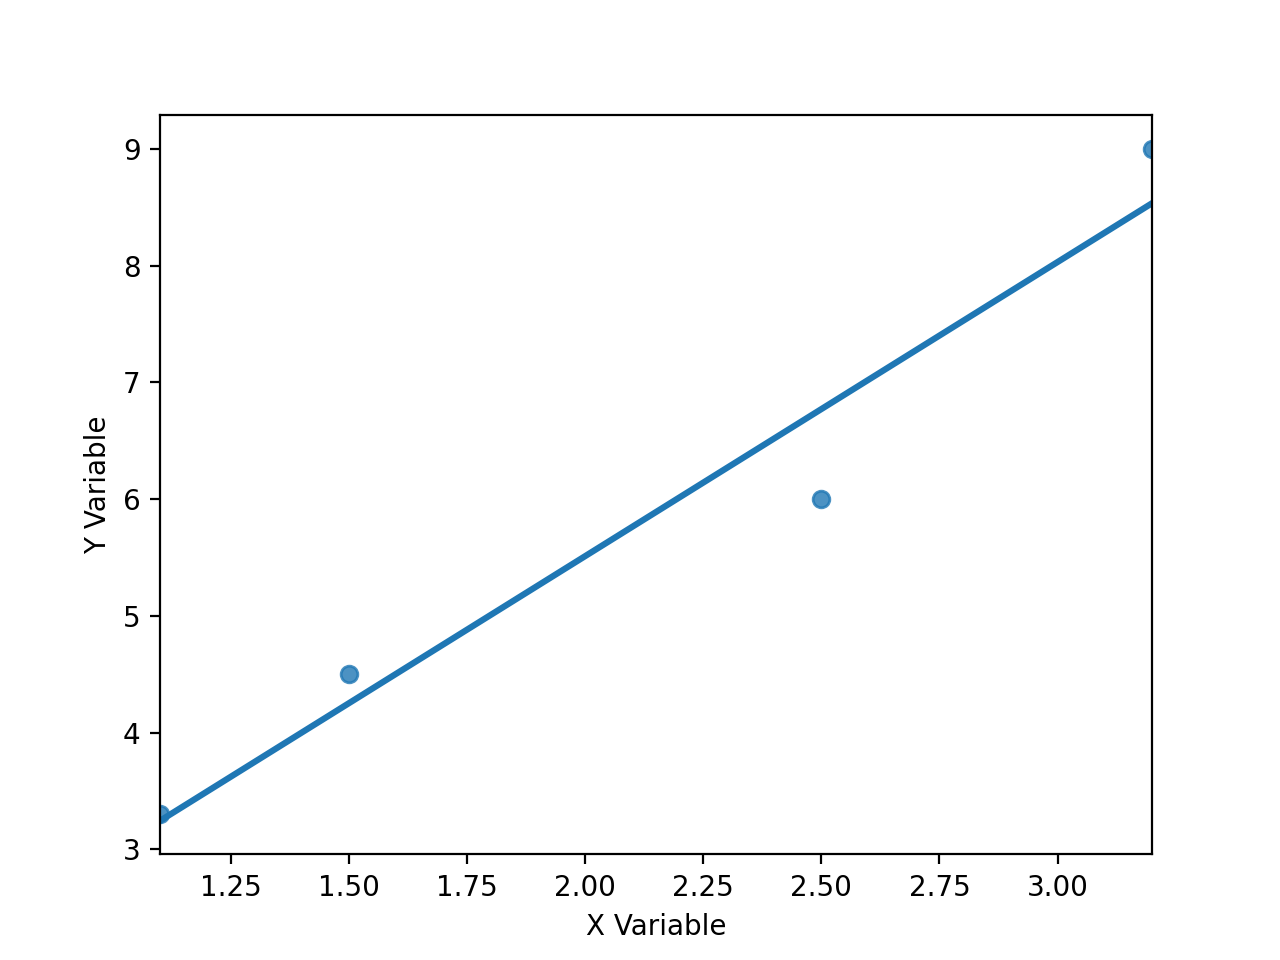
\includegraphics[width=0.5\textwidth]{mathematics/fig/linearRegression.png}}


\subsection{Multiple Regression}
Multiple regression is just linear regression done for more than one feature dimension. In general the problem it solves is of the form
\begin{align}
	\min_w||Xw-y||^2_2
\end{align}
Where $w$ is the weight vector, $x$ is the feature vector (including a term for the intercept) and $y$ is the label.

\subsection{Ridge Regression}
Ridge regression is a linear regression with an added penalty term proportional to the sum of the squared weights. This effectively prevents the model from becoming heavily dependent on a single weight and therefore is helpful in situations where the feature vectors are correlated (multicollinearity). The function to minimize is 
\begin{align}
	\min_w||Xw-y||^2_2 + \alpha||w||^2_2
\end{align}

\subsection{Lasso}
The LASSO (Least Absolute Shrinkage and Selection Operator) is designed to minimize the number of features the model is dependent on. The function it minimizes is 

\begin{align}
	\min_w\frac{1}{2n_{\textrm{samples}}}||Xw-y||^2_2 + \alpha||w||_1
\end{align}

Lasso can set weights to 0, while Ridge regression cannot.

\section{Hypothesis Testing}

\subsection{Confidence Intervals}
TODO
Also add calculation of confidence intervals of fit parameters.
Add confidence interval of a Gaussian

\subsection{P-Value}
The $p$-value is defined as the probability under the null hypothesis of obtaining a result equal to or more extreme than what was actually observed. The smaller the $p$-value, the more it tells investigators that the null hypothesis may not adequately explain the observation.


\subsection{A/B Testing}
See book \cite{grus}


\subsection{F-Test}
TODO

\section{Bootstrapping}
TODO


